\problemname{Tray Bien}

Andr\'{e} Claude Marzipan is the head chef at the French restaurant Le Chaud
Chien. He owns a vast number of baking trays, which come in two sizes: $1$ foot
by $1$ foot, and $1$ foot by $2$ feet. He stores them along $3$-foot deep
shelves of various lengths. For example, on a shelf that is $5$ feet long, he
might store baking trays in either of the two ways shown below:
\begin{center}
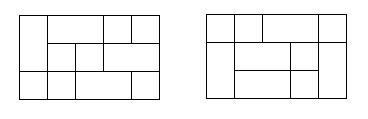
\includegraphics[width=0.5\textwidth]{trays.jpg}\\
Figure G.1
\end{center}

Of course, there are many more than just these two ways, and in his off hours
Andr\'{e} often wonders how many different ways he can place trays on a given
shelf. Andr\'{e} is a bit of \emph{un maniaque du rangement} (neat freak), so he
insists that the trays are always aligned along the two axes defined by the
shelf edges, that the edges of the trays are always $1$ foot multiples away from
any edge, and that no portion of a tray extends beyond the shelf. The matter is
complicated by the fact that often there are locations on the shelf where he
does not want to put any baking trays, due to leaks above the shelf, dents in
the shelf's surface, etc. Since Andr\'{e} is more adept at cuisine than
counting, he needs a little help.

\section*{Input}

The input consists of two lines: the first line will contain two integers $m$
$n$, where $1\le m\leq24$ indicates the length of the shelf (which is always
$3$-feet deep) and $n$ indicates the number of bad locations on the shelf. The
next line will contain $n$ coordinate pairs $x$ $y$ indicating the locations
where trays should not be placed, where $0<x<m$ and $0<y<3$. No location will
have integer coordinates and coordinates are specified to the nearest hundredth.
If $n=0$, this second line will be blank.
\newpage
\section*{Output}

Output the number of ways that trays could be placed on the shelf.

